\section{Research Results}
All results reported in this section are based on an average over 10 test runs, as described in Section \ref{sec:experiment_run}. We begin by presenting the performance, in terms of training and validation accuracy, of our approach. We then present a comparison of the average sparse categorical crossentropy loss for our approach and how this progressed during convergence. Finally, we report on the results of submitting our approach to the "Makerere Passion Fruit Disease Detection Challenge" \cite{zindi} and how it compares to other submissions.

\subsection{Accuracy}

Table \ref{tab:results} shows the average training and validation accuracy for classifying the fruits into classes and identifying bounding boxes. In addition, the standard deviation across the 10 runs is also reported.

\begin{table}[htbp]
\caption{Results in terms of accuracy.}
\centerline{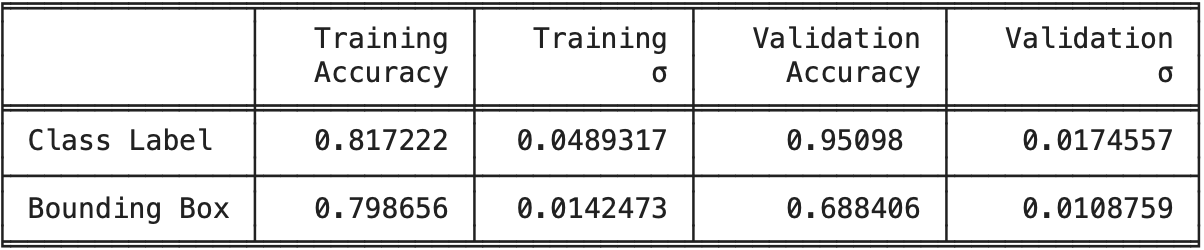
\includegraphics[width=0.5\textwidth]{report/5_results/results.png}}
\label{tab:results}
\end{table}

We note that, in the case of classifying fruit classes, validation accuracies were better than the accuracy achieved for training data. This may be as a result of over-fitting. However, the same is not true for the determination of bounding boxes; and so, we did not make alterations to the learning rate.

\subsection{Loss}
Figure \ref{fig:loss} shows the average sparse categorical crossentropy loss on the training and validation sets, for each approach.

\begin{figure}[htbp]
\centerline{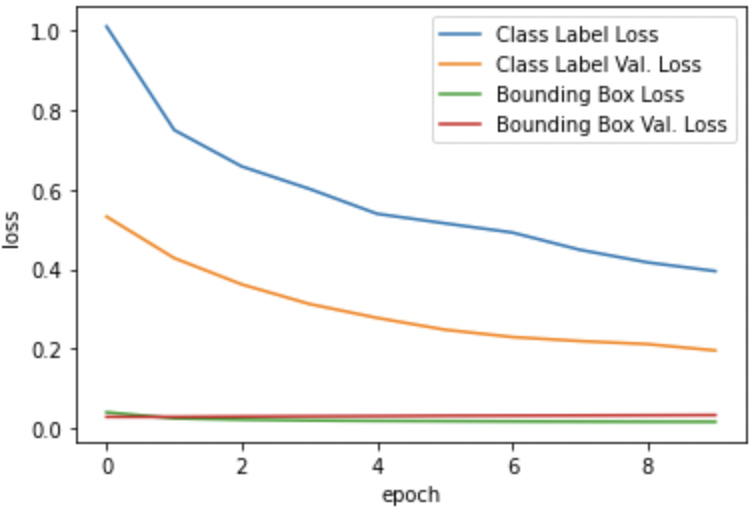
\includegraphics[width=0.4\textwidth]{report/5_results/loss.png}}
\caption{Progression of loss during training.}
\label{fig:loss}
\end{figure}

As can be seen, the loss for both the training and validation sets in the context of identifying bounding boxes was minimal from the start of training. This is due the the efficacy of ResNet50V2 \cite{ResNet50V2}, which had already been trained prior to the training of our model.

In addition, we can see that - in the context of classifying fruits, the network had not yet fully converged. This is likely because we had only trained the network for 10 epochs. It is also notable that the network seemed to generalse well in that validation loss was consistently lower than training loss for the classification of fruits.

\subsection{Comparison}
Upon submission to the "Makerere Passion Fruit Disease Detection Challenge" \cite{zindi}, our network received a score of around 0.30696. At the time of writing, this ranked it 121st on the leaderboard for the competition. It was also quite a ways of the leaders who had scored 0.90311.